\section{Overview}
\label{sec:overview}

\begin{figure}[t] 
  \centering 
  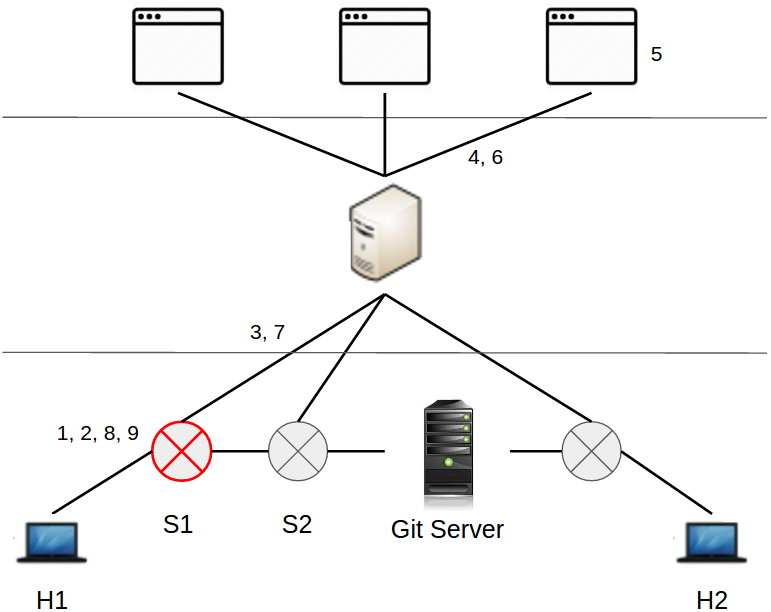
\includegraphics[width=3.3in]{img/overview.png}
  \caption{Overview of a reconnaissance attack abusing packet\_in
  messages.} 
  \label{fig:overview}
\end{figure}

Identifying network reconnaissance is an important piece of a defense 
in depth approach the network security. The information gathered during
network reconnaissance can lead to damage to the network and financial
losses. Therefore, reconnaissance activity is a strong indicator of a 
network breech and allows for administrators to respond before an 
adversary can carry out the rest of their attack. In this section, we 
first give a walkthrough of a previously undetected network 
reconnaissance attack from a compromised switch in a software defined network,
and then we propose an approach to detect this activity.

% how to perform network reconnaissance
As described in Section~\ref{sec:background} every packet not matching 
any flows installed in a switch's flow table will result in a switch 
sending a packet\_in message to the controller, which is then
processed by one or more applications. Once processed, the application
sends a flow\_mod to be installed in the switch's flow table dictating
what should be done with the packet and all packets matching the same
flow. Using this mechanism it is possible to infer information about the
network policy from the responses to packet\_in messages generated at a
switch. 

At a high level an adversary can perform network reconnaissance from a
compromised switch by treating the security and routing applications as
a black box, probing it with spoofed packets that generate packet\_in 
messages and learning the network policy from the resulting flow\_mod 
messages sent by the applications. To a naive application, these 
illegitimate packet\_in messages are indistinguishable from any other 
packet\_in message and processed normally. 

Figure~\ref{fig:overview} shows how an adversary can use packet\_in 
messages to discover the network connectivity in subnets whose traffic
does not flow through their compromised switch. In the following example
we walkthrough how an adversary, who compromised switch S1, can 
determine if host H2 can connect to the Git server. First the adversary 
generates a spoofed packet with source address H2 and destination address
of the Git server. In step 2, the adversary picks a spoofed source switch
port for the message before sending a packet\_in message to the controller
in step 3. Once receiving this message, the controller notifies all apps
listening for packet\_in events (step 4). Applications then process the 
packet (step 5) and send control messages to the controller (step 6).
After receiving a control message, the controller sends flow\_mod messages
to the switch installing the flow rule generated by the application (step 
7). Finally, in step 8, the adversary determines the network policy 
applied for the spoofed packet from the flow\_mod message. Optionally, an
adversary can take a ninth step to prevent the packet from being 
propagated throughout the network. In step 9,  the adversary drops the
spoofed packet at the switch and refuses to install the flow rule
generated by the application. This additional measure reduces the 
adversary's footprint within the network and gives a better chance at
staying in the network undetected.

% how to detect network reconnaissance
We now propose a solution to detect packet\_in abuse for network
reconnaissance of an SDN. First it is important to note this attack is
made possible because the controller and the apps often trust the data
reported by a switch and make no attempt to verify the legitimacy of the
reported data. Therefore, if each packet received from a switch is
verified, we can identify both a spoofed packet and the switch where the
packet was generated, with a few exceptions we mention in
Section~\ref{sec:disc}. 

The key identifying characteristic of network reconnaissance using 
packet\_in abuse is the adversary must spoof the event source port for
the packet\_in message. Using this characteristic, it is possible to
detect spoofed packet\_in messages by verifying the event source port
for packet\_in a message is the expected event port for a given source 
IP address in a packet. If the event source port does not match the
expected physical switch source port for a given packet then an alarm
can be raised alerting an administrator a reconnaissance packet has 
been discovered and a switch is potentially compromised. 

%% Challenges
The approach described above adequately provides a detection for
packet\_in message abuse, but it does not come without its challenges.
We briefly describe challenges faced by our approach here and then 
further address how we overcome these challenges in 
Section~\ref{sec:design}.

\begin{enumerate}
  \item \textbf{Detection Accuracy:} Since reconnaissance attacks may
    send only a few probes per day or even week, it is crucial that all
    probes are accurately detected to alert administrators of a network 
    intrusion. Additionally, if a large number of false positives are 
    present legitimate reconnaissance probes may go unnoticed by 
    administrators defeating the purpose of our defense.
  \item \textbf{Detection Time:} The quicker our solution is able to
    detect probe packets and raise an alarm for network administrators,
    the sooner actions can be taken to prevent the adversary's
    reconnaissance from being used in an attempt to exfiltrate data from
    the network.
  \item \textbf{Low Overhead:} Any defense implementing our proposed
    solution should not cause excessive overhead on network latency or
    throughput. If our solution is implemented in a real time network,
    even the smallest amount of overhead may deem our defense mechanism
    useless.
\end{enumerate}
